\section{Discussion and Limitations}\label{sec:discussion}

The evaluation is layer-level: it measures the forward and backward maps of a fixed cost on a synthetic crossing, on 1D normal forms, and on a controlled two-mode construction over 15 real LINEMOD frames, rather than the accuracy of a perception system. Detector-level ADD(-S)/ADD-S AUC, a learned front-end, and end-to-end training are outside the study, so the numbers characterise the layer and not a deployed pipeline. The forward pass inherits its globality from the enumerator, and completeness of the real-root enumeration is assumption (A2): the total-degree homotopy certifies the generic complex root count, not the missed-root rate of the multi-start Newton. The Laplace posterior mean is pulled toward the competing mode on real near-ties, where the hard argmin is accurate, so smoothing buys a well-defined gradient at the cost of pose accuracy. The constructed Choi--Lam cost is a valid symmetric matrix, but its realizability as the Gram matrix of an actual correspondence set remains open.

\subsection{Fold behaviour and continuity}

The $O(\tau)$ error of the Laplace approximation is non-uniform at a saddle-node (fold). There the mode count changes and a real-root-only Laplace sum is not even continuous. The exact smoothed posterior is smooth for every $\tau>0$ (Section~\ref{sec:laplace}); for the Laplace implementation the accuracy and continuity statements hold away from folds. Section~\ref{sec:fold6d} measures both faces: at $\theta=0$ the Laplace map is smooth (its jump decays linearly with FD slope $\approx502$ while the hard map's jump stays $2.86$), but a genuine fold sits at $\theta_f\approx1.31\times10^{-3}$, where that minimum dies, its weight reaches $0.122$, $\|d\phi\|$ peaks at $3529$, and the pose map steps by $0.31$. Smaller $\tau$ or more starts do not remove the step; the $\det(H+\tau^{1/3}I)$ regulariser reduces the derivative spike by a factor 24 and the near-fold gradient error from $2.9\times10^{-1}$ to $1.2\times10^{-2}$, but only halves the value step ($0.309\to0.107$). Two results explain why.

\begin{proposition}[Real-root proxies must jump]\label{prop:q5b}
Let $J_\theta$ undergo a standard codimension-1 fold ($A_2$) at $\theta_f$: on the side where they exist ($\theta\to\theta_f^+$), a secondary real minimum $q_+$ and a nearby saddle $q_-$ merge into $q_0$ (one Hessian eigenvalue $\lambda_1(q_+)\to0^+$, transverse Hessian $H_\perp(q_0)\succ0$, and a deeper minimum elsewhere with $J_0=J_{\theta_f}(q_0)>J_{\rm glob}$), and on the other side the real minimum is gone, so $K\to K-1$. Then any proxy that sums only over real local minima and gives the merging mode a positive regularised floor weight
\begin{equation}
\tilde w_+^{\rm reg}(\theta_f^+)=\frac{(2\pi\tau)^{3/2}}{\sqrt{\det(H_++\eta(\tau)I_3)}}\,e^{-J_0/\tau},
\label{eq:floorweight}
\end{equation}
with the scale-matched floor $\eta(\tau)=c_0\tau^{1/3}$, forces the smoothed loss $\bar\ell_{\rm reg}$ to jump at $\theta_f$ (with $Z_{\rm rest}$ the Laplace partition function of the other modes):
\begin{equation}
\begin{split}
&\lim_{\theta\to\theta_f^+}\bar\ell_{\rm reg}-\lim_{\theta\to\theta_f^-}\bar\ell_{\rm reg}\\
&\quad=\frac{\tilde w_+^{\rm reg}(\theta_f^+)}{\tilde w_+^{\rm reg}(\theta_f^+)+Z_{\rm rest}(\theta_f)}\big(\ell(q_0)-\bar\ell_{\rm rest}(\theta_f)\big)\neq0,
\end{split}
\label{eq:jump}
\end{equation}
and for $\eta=c_0\tau^{1/3}$ the jump is $\Theta\big(\tau^{1/3}e^{-(J_0-J_{\rm glob})/\tau}\big)$.
\end{proposition}

The jump is exponentially small only when $J_0-J_{\rm glob}\gg\tau$, and stays $O(1)$ when $J_0-J_{\rm glob}=O(\tau)$; at any finite $\tau$ it is nonzero. This is a necessity statement about real-root proxies, and it is why $0.309\to0.107$ does not go to zero.

\begin{proposition}[Complex-conjugate roots and the Scorer continuation]\label{prop:q5c}
The 40-root action-matrix solver carries the merged pair through the fold as a complex-conjugate pair. In the normal form
\begin{equation}
J_\theta(u,v)=J_0(\theta)+\tfrac12v^\top H_\perp(\theta)v+\tfrac{c_3(\theta)}{6}u^3-\alpha(\theta)u
\label{eq:normalform}
\end{equation}
with $c_3>0$, $\alpha(\theta_f)=0$ and $\alpha'(\theta_f)>0$ (Gromoll--Meyer splitting), define the invariants $J_0=(J(q_+)+J(q_-))/2$ and $\zeta(\theta,\tau)=\alpha(\theta)\big(2/c_3(\theta)\big)^{1/3}\tau^{-2/3}$, and the semi-line Airy (Scorer) integral
\begin{equation}
\mathcal{S}(\zeta)=\int_0^{+\infty}e^{-s^3/3+\zeta s}\,ds,
\label{eq:scorer}
\end{equation}
which is entire with $\mathcal{S}(0)=\Gamma(1/3)/3^{2/3}\approx1.2879$. Replacing the two real-root weights by the single continuation
\begin{equation}
\begin{split}
\tilde w_{\rm fold}(\theta,\tau)={}&\frac{2\pi\tau}{\sqrt{\det H_\perp(\theta)}}\,\tau^{1/3}\Big(\frac{2}{c_3(\theta)}\Big)^{1/3}\\
&\times e^{-J_0(\theta)/\tau}\,\mathcal{S}\big(\zeta(\theta,\tau)\big),
\end{split}
\label{eq:foldweight}
\end{equation}
gives a map that is $C^\infty$ across $\theta_f$ with zero value jump, because $(J_0,\alpha,c_3,H_\perp)$ are symmetric functions of the characteristic polynomial and $\mathcal{S}$ is entire. For $\zeta\gg1$ it reduces to the ordinary 3D Laplace weight of the surviving minimum, $\tilde w_{\rm fold}=\tilde w_{\rm Lap}(q_+)\big(1+O(\tau/\Delta J_{\rm bar})\big)$; for $\zeta\ll-1$ it decays smoothly, $\mathcal{S}(\zeta)=|\zeta|^{-1}\big(1+O(|\zeta|^{-3})\big)$.
\end{proposition}

\textbf{The continuation at the invariant level.} The 6D fold at $\theta_f=1.3185\times10^{-3}$ is tracked on both sides (real minimum/saddle pair and the complex-conjugate pair), the four invariants $(J_0,\alpha,c_3,H_\perp)$ and $\mathcal{S}(\zeta)$ are continuous across it, and the measured pose jump is $1.21\times10^{-2}$ versus $3.04\times10^{-1}$ (standard) and $1.07\times10^{-1}$ ($\tau^{1/3}$), i.e.\ at the smooth-map derivative scale ($|d\phi|\sim6\times10^2$, jump/step $6.0\times10^2$ versus $1.5\times10^4$). The identification of the measured invariants with the normal form is leading-order (the quartic's fourth-order coefficient is $\approx8.3$), and this 6D fold is shallow ($\Delta J\sim10^{-6}\ll\tau$), so the Scorer weight is far from its 3D-Laplace limit \emph{at} the fold. The main table reports the real-root-only layer, whose step is the one Proposition~\ref{prop:q5b} predicts.

\begin{table}[t]
\centering
\caption{Scorer continuation vs real-root proxies at the 6D fold ($\theta_f=1.3185\times10^{-3}$, $\tau=0.01$, grid $\theta_f\pm10^{-4}$ step $2\times10^{-5}$). \emph{jump} is the largest consecutive pose difference; a genuine step keeps \emph{jump/step} growing under refinement, a smooth map has \emph{jump/step} at the $|d{\rm pose}|$ scale ($\sim6\times10^2$). The 1D three-way check reproduces $0.867/0.497/0.3391$ to $\le1.6\times10^{-4}$.}
\label{tab:scorer}
\footnotesize
\setlength{\tabcolsep}{4pt}
\begin{tabular}{@{}l l l l@{}}
\toprule
variant & max jump & jump / step & $K$ on grid\\
\midrule
standard real-root Laplace & 3.04e-01 & 1.52e+04 & 3--4\\
$\det(H+\tau^{1/3}I)$ regularized & 1.07e-01 & 5.34e+03 & 3--4\\
Scorer continuation & 1.21e-02 & 6.03e+02 & 4\\
\bottomrule
\end{tabular}
\end{table}

\begin{figure*}[t]
\centering
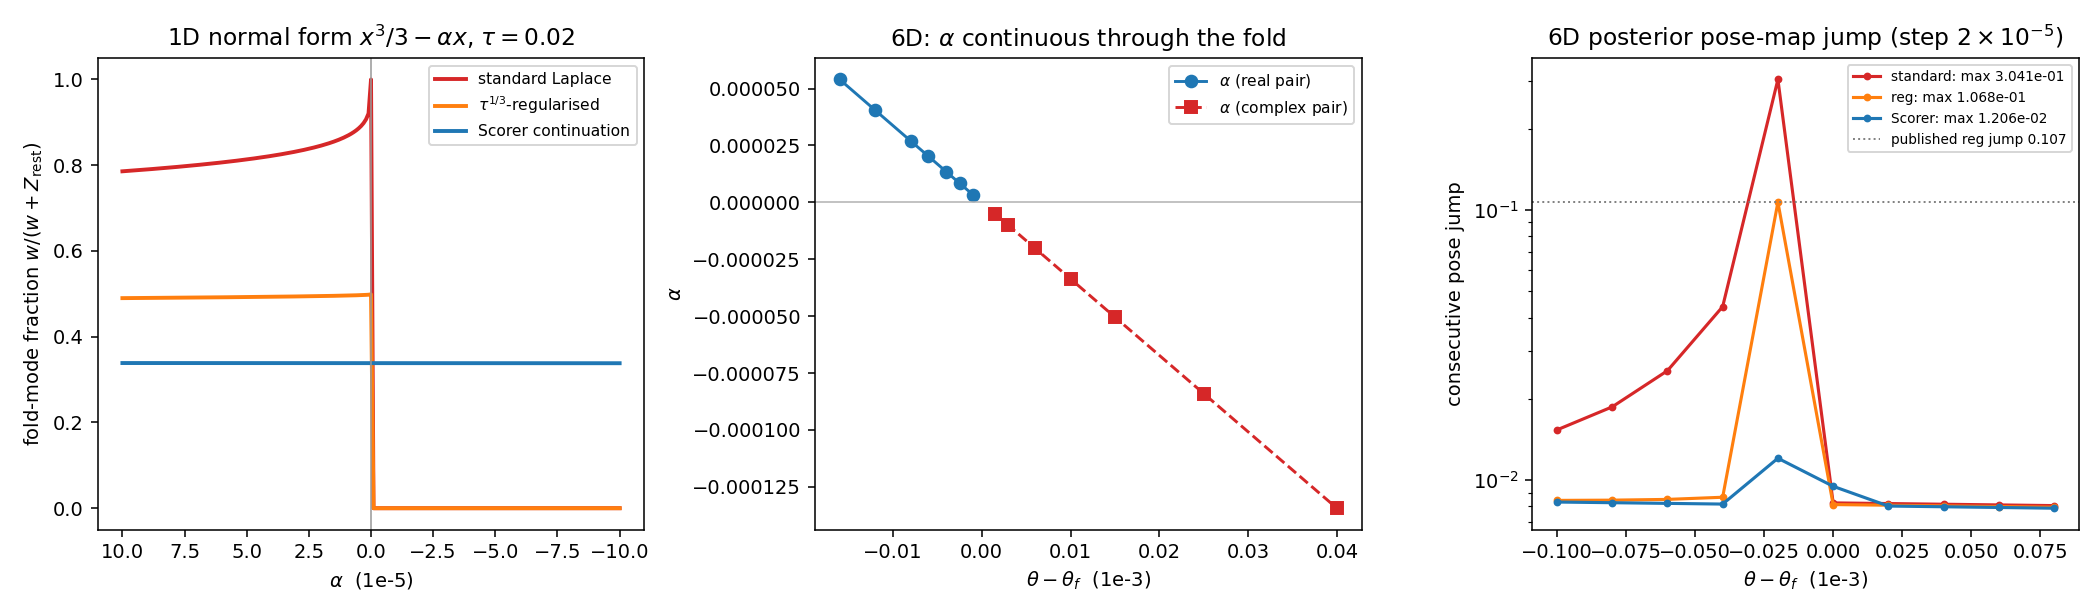
\includegraphics[width=0.80\textwidth]{scorer_fold.png}
\caption{The Scorer continuation at a fold. \textbf{Left:} the 1D normal form $x^3/3-\alpha x$ at $\tau=0.02$; the fold-mode weight fraction is discontinuous for the standard Laplace sum, jumps from $0.4959$ to $0$ for the $\tau^{1/3}$-regularised volume factor, and is continuous ($0.33838\to0.33834$) for the Scorer continuation. \textbf{Middle:} the 6D fold at $\theta_f=1.3185\times10^{-3}$; the invariant $\alpha$ is tracked through the fold, continuous across the real-pair/complex-pair switch. \textbf{Right:} the largest consecutive posterior pose jump against $\theta-\theta_f$: the standard map spikes to $3.04\times10^{-1}$, the regularised one to $1.07\times10^{-1}$, and the Scorer continuation peaks at $1.21\times10^{-2}$, at the smooth-map derivative scale.}
\label{fig:scorer}
\end{figure*}

The continuity claim is tested by grid refinement (staggered grids, half-width $10^{-4}$, step $d\in\{4\times10^{-5},\ldots,2.5\times10^{-6}\}$): the Scorer \emph{jump/d} stays $404.3,404.2,404.0,403.7,403.3$ over a $16\times$ range of $d$ (no numerical floor at $d=2.5\times10^{-6}$), whereas the standard map's \emph{jump/d} grows from $7.6\times10^{3}$ to $2.1\times10^{5}$ and the regularised one from $2.7\times10^{3}$ to $4.4\times10^{4}$ (a constant step). The fold neighbourhood therefore requires the Scorer continuation, or a local numerical integral over the merging pair, for a continuity claim.



\subsection{Future work}

Extending the evaluation to a learned front-end, to detector-level ADD(-S)/ADD-S AUC on LINEMOD/LINEMOD-Occlusion and to UTIAS In-The-Dark, and comparing against SDPR and EPro-PnP, are left for future work. A per-instance certified real-root count, a batched GPU forward, learned temperature calibration and third-derivative contraction for the full Laplace KL are the natural next steps.
